\documentclass[a4paper,8pt,hyperref, twocolumn]{article}

\title{\bfseries \Large Cavity-enhanced second harmonic generation in a silica whispering-gallery microresonator}
%\author{\normalsize  Xueyue Zhang}
\date{\normalsize \today}

\usepackage[left=16mm,right=16mm, bottom = 16mm, top=20mm]{geometry}
\usepackage{upgreek}
\usepackage{hyperref}
\usepackage{booktabs}
\usepackage{tabularx}
\usepackage{xtab}
\usepackage{graphicx}
\usepackage{listings}
\usepackage{url}
\usepackage{amsmath}



\lstset{
	flexiblecolumns,
	basicstyle = \sffamily,
	keywordstyle = \bfseries,
	commentstyle = \rmfamily\itshape,
	stringstyle = \ttfamily
}

\hypersetup{
colorlinks=false}



%\pagestyle{myheadings}
%\markright{Name: Xueyue Zhang, GTID: 903181650}

\bibliographystyle{unsrt}

\begin{document}

\maketitle

%\section{Introduction}

%[Literature; origin, set-up, phase-matching, advantages: low pump power, continuous wave, possible applications and impacts]

Centrosymmetric materials ... most significant application: surface probe... surface response is intrinsically weak, so several methods are used to enhanced surface SHG (e.g. plasmonic)... cavity boosts the intensity of light, making it a good platform for nonlinear optics...cavity enhanced SHG... Recently, SHG with bare silica cavity (Asano OL)...

Here, second harmonic, originating from symmetry breaking at the surface and bulk multipole response (fig.\ref{pic:Fig1} \textbf{b}), is observed under the continuous wave pump below 1 mW in a WGM microsphere made of centrosymmetric material. 
An unprecedented conversion efficiency of 4$\times10^{-4}$W$^{-1}$ benefits from doubly resonant enhancement [CHECK] of ultrahigh $Q$ modes (phase-matching condition), which is achieved by dispersion engineering including thermal effect, optical Kerr effect and geometric control of cavity. 

% Apart from the compensation of cavity mode dispersion[], Additionally, the collecting efficiency of SH signal is significantly increased with the incorporation of a signal tapered fiber. 
The work paves the way for low power and continuous-wave SH sensing. The combination of resonant enhancement and silica surface may enable a series of nonlinear sensitive detection. [BROAD BAND FREQUENCY CONVERSION+SURFACE SENSING]
%\section{Experimental set-up and observation of second harmonic signal}
%[Explain the set-up and how to collect the signal; show the typical spectra and corresponding experimental conditions; explain why other nonlinear processes are absent; f1f2 comparison and conditions]

In the experiment, a silica microsphere (diameter [\~] $62$ $\upmu$m) 
is pumped through a tapered optical fiber (waist diameter around $1$ $\upmu$m) at $1550$ nm band \cite{knight1997phase, cai2000observation}, as shown in fig.\ref{pic:Fig1} \textbf{a}. To collect SH signal efficiently, a second fiber taper (waist diameter around 0.5 $\upmu$m) designed for 780 nm band is incorporated into the system. The intrinsic quality factor (Q) for the pumped cavity mode is $4.8\times10^7$. %When the signal tapered fiber is near the microsphere to couple SH signals, the effective intrinsic Q (including the intrinsic loss and loss induced by the signal fiber) decreases and a typical value is $3.6\times 10^7$.%The signals collected by the signal tapered fiber are sent into an electron-multiplying CCD (EMCCD) to extract the spectra.
% The EMCCD and the pump laser are placed at the same side of the microsphere considering the linear momentum conservation requirement in SHG\cite{carmon2007visible, kozyreff2008whispering}.
% A tapered fiber phase-matched at the telecommunication band couples the pump into the microsphere. This tapered fiber is not able to collect the second harmonic signal efficiently due to phase mismatch at around 780 nm and the high radial order of the second harmonic mode\cite{carmon2007visible}. To overcome this problem and collect weak second harmonic signals, another tapered fiber (signal tapered fiber) designed to achieve phase matching condition at second harmonic wavelength is fabricated together with the pump tapered fiber and incorporated into the system as is shown in Fig.\ref{pic:Fig1}a. The tapered fibers can reach critical coupling simultaneously at around 1555 nm and 777 nm. 
% A fiber coupler split 10\% of the pump power from the laser into a power meter to monitor the input power. 
Figure \ref{pic:Fig1}\textbf{c} shows a typical SH spectrum from the electron-multiplying CCD (EMCCD) and the corresponding pump spectrum from the optical spectrum analyzer (OSA). The SH signal of $777.75$ nm appears when pumped at $1555.14$ nm, which deviates only $0.023$\% from the expected wavelength, falling into the resolution tolerance of OSA and EMCCD.
Note that stimulated Raman scattering and parametric oscillation do not occur because their thresholds are above the pump power in the experiment% \cite{spillane2002ultralow, kippenberg2004kerr}. 
Third harmonic generation is also absent due to the phase mismatch in the nonlinear optical process.
% between the mode and its third harmonic modes\cite{carmon2007visible}. 
%Third harmonic signals  collected by the signal fiber are also observable when pumped at some specific modes [need figure?]. 
[e, ->d]
Moreover, SH signals arise in the full range when cavity modes are pump from $1545$ nm to $1565$ nm, as shown in Fig.\ref{pic:Fig1}d.
Thanks to the plethora of modes in the microsphere, SH signals arise in , which is 
Using the signal fiber, an SH signal with a power of 5 nW (shown in Fig.\ref{pic:Fig1}c) is collected at the pump wavelength of 1561.3 nm. 
%The SH power is calibrated from the EMCCD spectra to represent the power in the signal fiber near the microsphere. 
In order to compare the collecting efficiency, the pump tapered fiber is connected directly to the EMCCD and the coupling between the pump fiber and the microsphere is optimized to maximize the collected SH power. The SH signal is still observable but the maximum power is only 0.36 nW, which is more than 13 times weaker than the SH power collected by the signal fiber.

The SH signal is only present when the pump light is in the mode (judging from the transmission). Because of thermal bistability\cite{carmon2004dynamical}, the pump light can be out of the mode when tuning the wavelength to blue side but in the mode when tuning in the opposite direction. At the same wavelength, only the in-mode pump can produce the SH. And the SH signal is always absent when the microsphere is moved far from the pump fiber, which also help to eliminate the possibility of spurious signals created by the second order diffraction of the EMCCD grating.

\begin{figure*}[!ht]
\centering
%\captionsetup{singlelinecheck=no, justification = RaggedRight}
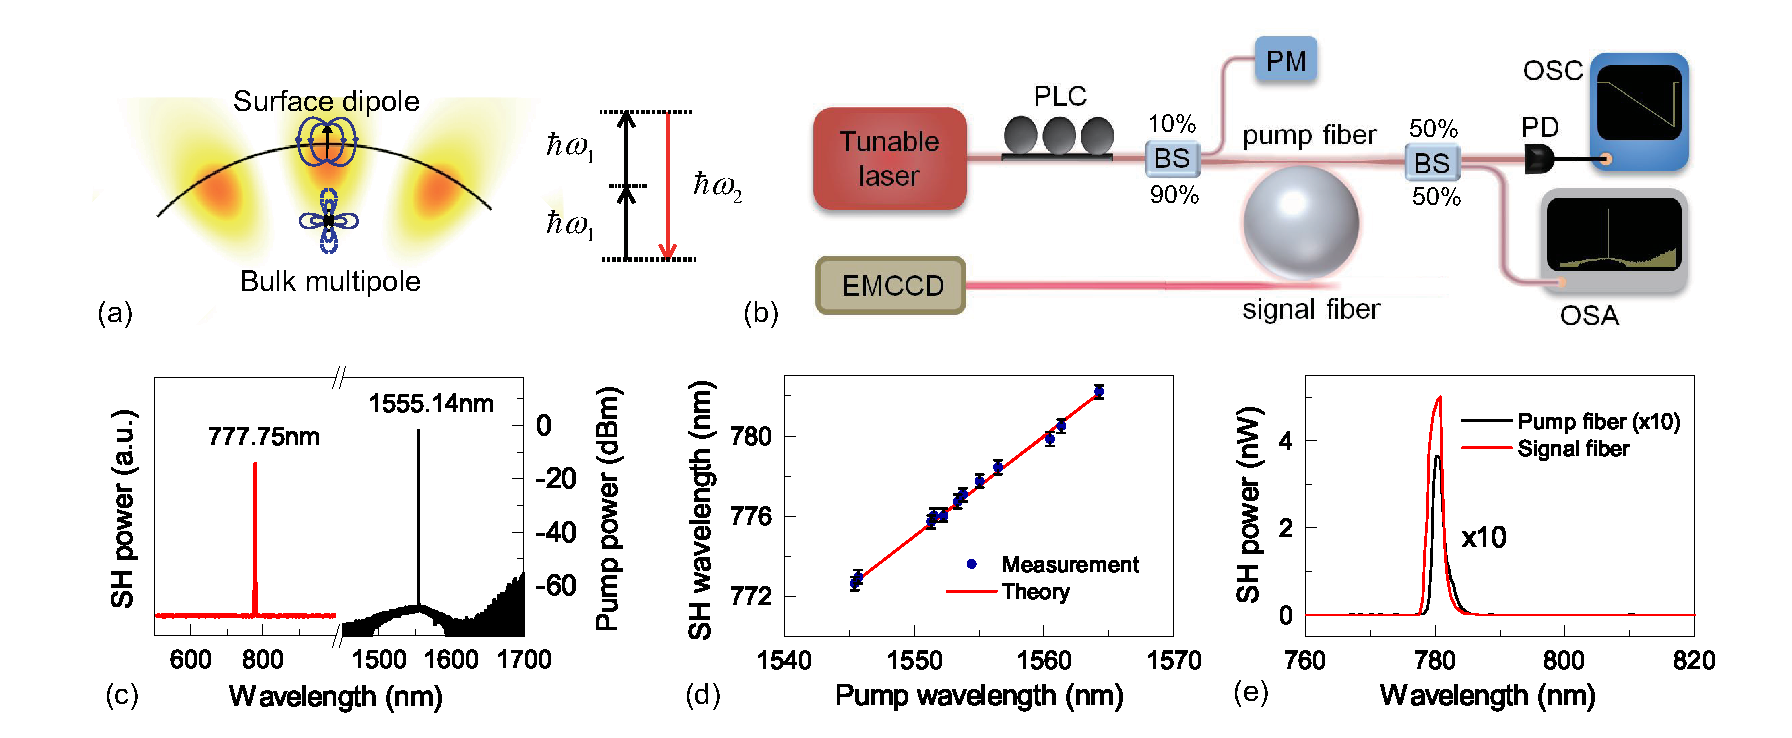
\includegraphics[width=18cm]{Fig1.eps}
\caption{\textbf{Experimental set-up and observation of cavity-enhanced SH signals. a, }The pump light from a tunable laser around 1550 nm is coupled into a silica microsphere through a tapered fiber, and a second fiber is used to collect the SH signal. OSC: oscilloscope. OSA: optical spectrum analyzer. PLC: polarization controller. BS: beam splitter. EMCCD: electron-multiplying CCD. \textbf{b, }SH is generated from the surface dipole response and the bulk multipole response in a WG microsphere. \textbf{c, }Measured SH spectrum (red) and the corresponding pump spectrum (black). \textbf{d, }Comparison of SH power collected by signal fiber and pump fiber (10 times magnified). \textbf{e, }Measured SH wavelengths versus the corresponding pump wavelengths when different modes are pumped.}
\label{pic:Fig1}
\end{figure*}

%The signal tapered fiber in this set-up is critical to collect SH signals efficiently. 


%\section{Thermal effect and Kerr effect assisted phase-matching}
%[Prerequisite phase matching (higher order radial modes) and its problems; P2-P1 relation and how to enhance SH signals; mechanisms for assisted phase-matching; results: dependence on detuning and power; comparison with other SH and silica sphere TH.]

The dependence of SH power on pump power can be derived from coupled mode equations\cite{haus1991coupled}.
\begin{equation}
P_2 = \frac{4|g|^2Q_2\eta_2/\omega_2}{4Q_2^2(2\omega_p/\omega_2-1)^2+1}\frac{16Q_1^2\eta_1^2P_1^2/\omega_1^2}{[4Q_1^2(\omega_p/\omega_1-1)^2+1]^2},
\label{eq:P2P1}
\end{equation}
where the subscripts 1, 2 represent the pumped mode and SH mode respectively. $P_i$ ($i=1, 2$)is the power in the corresponding tapered fiber near the microsphere, $g$ is a coupling coefficient between two modes, which will be looked into in the next section. $Q_i$ is the total quality factor, $\omega_i$ is the mode frequency and $\omega_p$ is the pump frequency. $\eta_{i}=Q_i/Q_{ie}$ is the coupling factor and $Q_{ie}$ is the external quality factor. The pump power depletion is ignored due to the weak second order nonlinear effect in silica. The enhancement of SH power by ultrahigh-Q microresonator is obvious in eq.(\ref{eq:P2P1}). 

The ultrahigh Q also presents a challenge to phase matching, which corresponds to double on-resonance conditions ($\omega_p = \omega_1, 2\omega_p = \omega_2$) in a microresonator\cite{carmon2007visible, kozyreff2008whispering, xu2008second, farnesi2014optical}. SH or TH modes with higher order radial number have been proposed or used to compensate the material and geometric dispersion\cite{carmon2007visible, kozyreff2008whispering, farnesi2014optical}. For SHG, a silica microsphere with a diameter of 60$\upmu$m gives rise to good phase-matching between a fundamental mode near 1550nm and an SH mode with radial number $q_2=2$. But due to the discrete distribution of modes, the mode with smallest phase mismatch can reduce the SH power by a factor of $10^{-6}$. This phase matching method is also extremely sensitive to the size of microresonators. A deviation of 3\% in diameter can lead to a reduction of SH power by nearly 4 orders of magnitude. It is difficult to control the size of a microsphere precisely in the experiments. Therefore, other mechanisms are required to achieve phase matching. Thermal effect and Kerr effect have been utilized to compensate the dispersion in microresonator-based frequency comb generation\cite{del2011octave, herr2014temporal}. These effects can also help to achieve phase matching in SHG. Both of the two effects lead to a red shift of the mode frequency \cite{ilchenko1992thermal, treussart1998evidence,  carmon2004dynamical, fomin2005nonstationary} and there is no need to distinguish them because the focus is steady state continuous wave emission. 

Fig.\ref{pic:Fig2}a explains the mechanism of thermal and Kerr assisted phase matching process. When the pump power is weak and the mode red shift is negligible (cold cavity), the pumped and SH modes even with higher radial order usually cannot be on resonance with the pump light and its SH simultaneously. When the pump power is large enough, the pumped mode shifts more to the red side with increasing intra-cavity power. Tuning the pump frequency from the cold cavity mode to the red side can decrease the detuning $\omega_p-\omega_1$ and increase intra-cavity power, thus making the triangular resonance shape \cite{carmon2004dynamical}. The SH mode also experiences a red shift from cold cavity frequency when intracavity power is large. If the speed of red shift is different for the pump light SH and the SH mode, then it is possible for them to be on resonance in the process of tuning the pump frequency. The SH power will reach a peak value at the on-resonance pump frequency but decrease rapidly after the frequency. The SH power is weak compared with the input power so that its thermal and Kerr effects are negligible in this process.

\begin{figure*}[!ht]
\centering
%\captionsetup{singlelinecheck=no, justification = RaggedRight}
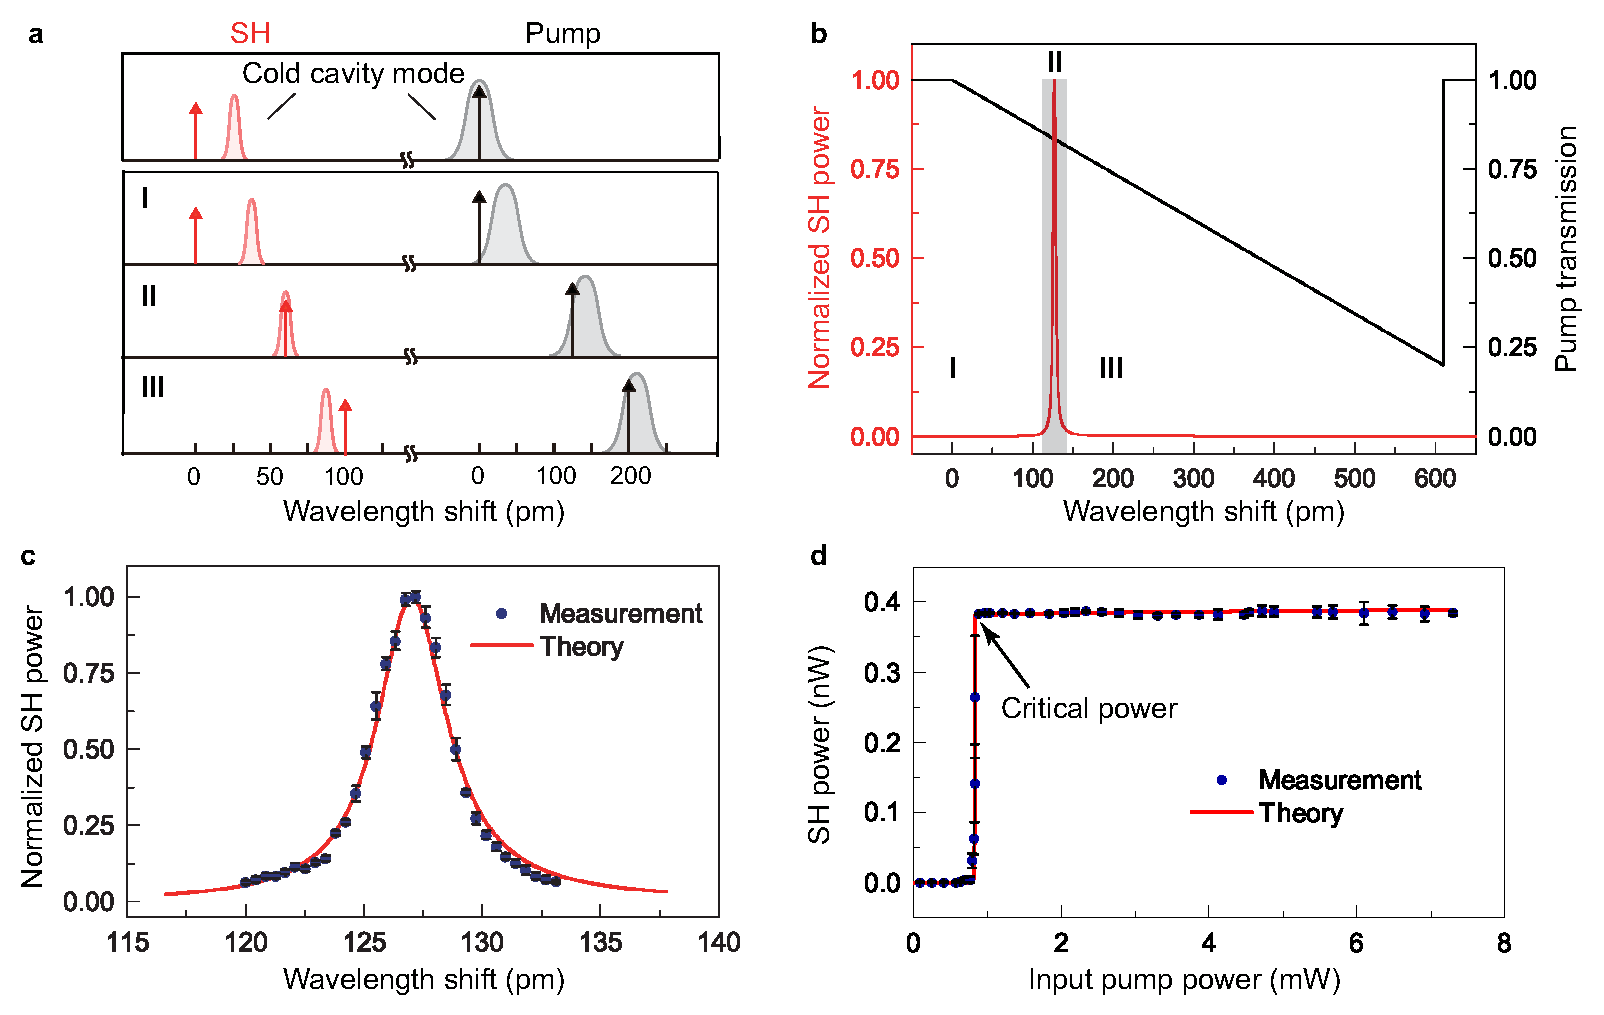
\includegraphics[width=17cm]{try_ed3.eps}
\caption{\textbf{Thermal effect and Kerr effect assisted phase-matching. a, }Schematic of the phase-matching process. Detuning here is the wavelength relative to the cold-cavity wavelength of the pumped mode (to half of this wavelength for SH detuning). The black (red) arrow represents the detuning of the pump light (its SH). The gray (red) Lorentzian line represents the pumped mode (SH mode). 1-3 show three states with increasing pump wavelength but the same input power. \textbf{b, }Normalized SH power and the pump transmission at different pump wavelength detuning. 1-3 correspond to the three states in panel \textbf{a}. The gray area is enlarged in panel \textbf{c} as the theoretical red line. \textbf{c, }SH power versus pump detuning with the input power of 4.46mW. \textbf{d, }The dependence of maximum SH power at all the pump detuning on the input power.}
\label{pic:Fig2}
\end{figure*}

When the mode in Fig.\ref{pic:Fig1}b is pumped with an input power of 4.46 mW, the SH power exhibits a clear peak at the pump wavelength of 1555.14 nm, which is shown in fig.\ref{pic:Fig2}c. The red shift of the SH mode is proportional to the intra-cavity power, which is proportional to the pump light detuning from the cold cavity frequency. It means $\Delta \omega_2 = D_{12}\Delta \omega_p$, where $\Delta \omega_2$ is the SH mode frequency shift, $\Delta \omega_p$ is the pump light detuning and $D_{12}$ is the proportionality coefficient.  Using this relation and eq.(\ref{eq:P2P1}), the experimental parameters can be fit by the theory to be $Q_2\times(2-D_{12})=8.57\times 10^5$.

The thermal and Kerr assisted phase matching makes the SH power depend strongly on the pump frequency, which also determines the intra-cavity pump power. At a certain pump frequency (the mode frequency is still at the red side of the pump), when the input power increases, the intra-cavity power also tends to increase, which pushes the mode frequency to the redder side. The pump frequency remains unchanged so that the detuning $\omega_p-\omega_1$ increases to lower the coupling efficiency of the input power into the cavity. Therefore, the intra-cavity pump power increases more slowly than the increase of input pump power. 

The dependence of SH power and intra-cavity power on the pump frequency gives rise to a novel relation between the SH power ($P_2$) and the input pump power ($P_1$). When $P_1$ is not large enough for the pump SH to catch the SH mode before the pump frequency catches the mode frequency, the SH mode cannot be on resonance at any pump frequency and the SH power is small because of the ultrahigh Q. When $P_1$ reaches a critical power so that the pump SH and the pump frequency catch the two modes simultaneously, the two denominators in eq.(\ref{eq:P2P1}) reach the smallest value of 1, which gives rise to an efficient SHG. When $P_1$ further increases from the critical power, the intra-cavity power increases slowly so that the SH-on-resonance frequency also moves slowly, therefore, when the pump SH is on resonance with the SH mode, the intra-cavity pump power and the corresponding SH power does not change as rapidly as the input pump power. We also measured the SH power versus input pump power with the mode in Fig.\ref{pic:Fig1}c. At each input pump power, the pump wavelength range from the cold cavity mode (1555.02nm) to the pump on-resonance wavelength was searched for the maximum SH output power. And the maximum SH power against input pump power is shown in Fig.\ref{pic:Fig2}d. The critical input power is fitted to be 832.5$\upmu$W and the corresponding SH power is fitted to be 381pW. Eq.(\ref{eq:P2P1}) and $\omega_1 = \omega_{10}-B_{11}|\alpha_1|^2$ \cite{carmon2004dynamical}, $\omega_2 = \omega_{20}-B_{12}|\alpha_1|^2$ are used to fit the experimental data, where $\omega_{i0}$ is the mode frequency in the cold cavity, $|\alpha_1|^2$ is normalized to the intra-cavity power of the pumped mode and $B_{1i}$ is the coefficient of intra-cavity power induced frequency shift. The parameters related to the pumped mode can be extracted from the measurements. 

\begin{figure*}[!ht]
%\centering
%\captionsetup{singlelinecheck=no, justification = RaggedRight}
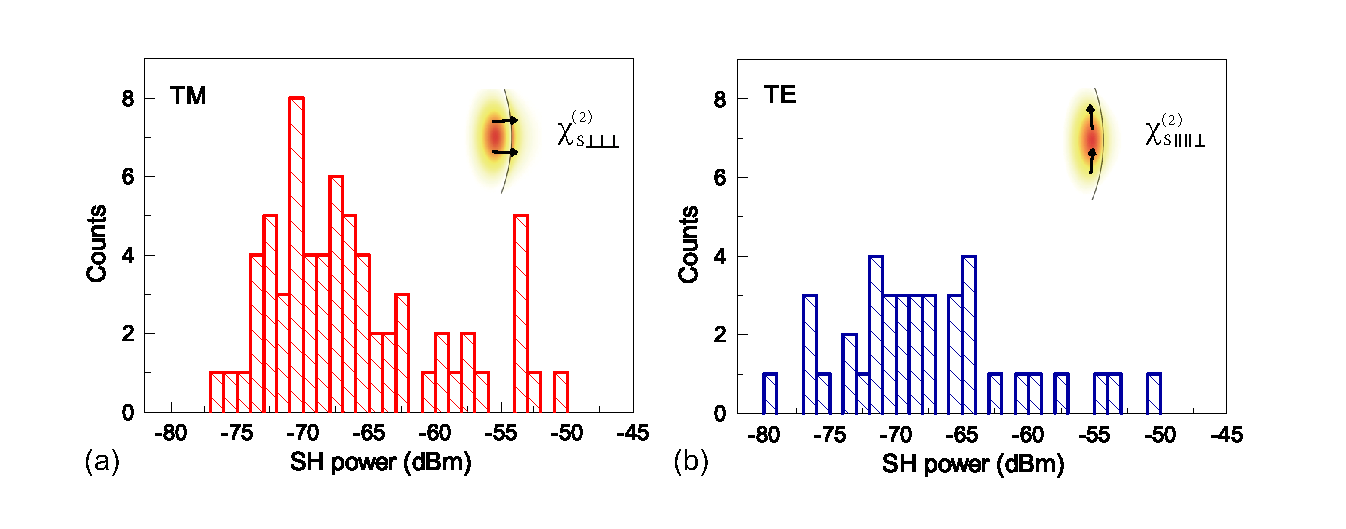
\includegraphics[width=18cm]{Fig3.eps}
\caption{\textbf{SH power histogram with different pump polarization. a, } TM and \textbf{b,} TE modes are pumped to generate SH respectively. Insets: Field amplitude distribution and the direction of the electric field (black arrow).}
\label{pic:Fig3}
\end{figure*}

In the THG experiments in silica microresonators\cite{carmon2007visible, farnesi2014optical}, the phase mismatch curve is flat for high order radial modes, and the shift speed of the pump TH frequency and the TH frequency mode may be similar. Consequently, the high order radial modes induced phase matching may play a major role so that the $P_1^3$ relation can be observed. Microresonator SHG in other materials usually use different phase matching strategy to achieve broad band or tunable phase matching, e.g. quasi-phase-matching [cite more later]...The quality factor is also moderate so that the thermal effect and Kerr effect do not manifest themselves in the SHG process.

It is also possible to measure the explicit $P_2 \propto P_1^2$ dependence by introducing another degree of freedom to manipulate the SH mode frequency. For example, a control light can be coupled into another mode to change the intra-cavity power and thus achieving the double on-resonance condition at various input pump power. The specific measurement plan is beyond the scope of this [letter?] and is still under investigation.


%\section{Origin of second order nonlinearity}



%[Theory for surface \& bulk 2nd nonlinearity; relationship with polarization]

Silica is a centrosymmetric material in which the electric dipole induced second order nonlinearity is forbidden (see \cite{boyd2003nonlinear} for reference). Surface symmetry broken and bulk multipole become the major sources of second order nonlinearity (see \cite{heinz1991second} for review). 




Using the Helmholtz equation and the relation between electric field and nonlinear polarization, the coupling coefficient induced by surface nonlinear response is
\begin{equation}
g_{s0} = 2i\frac{\omega_1^2}{\omega_2n^2}\frac{\int_{\mathrm{surface} } \mathbf{E}_{02}^*:\upchi^{(2)}_s:\mathbf{E}_{01}\mathbf{E}_{01} d\mathbf{S}}{\int |\mathbf{E}_{02}|^2 d\mathbf{V}}
\end{equation}
where $n$ is the refractive index, $\upchi^{(2)}_s$ is the surface nonlinear susceptibility, and $\mathbf{E}_{0i}(\mathbf{x})$ is the  normalized electric field so that $\alpha_i\mathbf{E}_{0i}(\mathbf{x})$ represents the complete electric field. 

The bulk multipole nonlinear polarization can be written as $\mathbf{P}_\gamma =  \gamma\nabla(\mathbf{E}\cdot\mathbf{E})$ and $\mathbf{P}_\delta =  \delta(\mathbf{E}\cdot\nabla)\mathbf{E}$, where $\gamma$ and $\delta$ are the nonlinear coefficients. The first term represents a longitudinal wave and can couple with the SH only at the surface. Therefore it can be incorporated into an effective surface susceptibility $\upchi^{(2)}_s = \upchi^{(2)}_{s0}+\upchi^{(2)}_{s,\gamma}$\cite{heinz1991second}. The coupling coefficient induced by the second term can be written as % $a'$
\begin{equation}
g_b =  2i\frac{\omega_1^2}{\omega_2n^2}\frac{\int \delta\mathbf{E}_{02}^* \cdot (\mathbf{E}_{01}\cdot\nabla)\mathbf{E}_{01} d\mathbf{V}}{\int |\mathbf{E}_{02}|^2 d\mathbf{V}}
\label{eq:gb}
\end{equation}
The total coupling coefficient between the two modes is $g = g_s+g_b$. 

There are three non-zero components $\upchi_{\perp \perp \perp}$, $\upchi_{\parallel \parallel \perp}$ and $\upchi_{\perp \parallel \parallel}$ in the surface second order susceptibility tensor of fused silica.  $\upchi_{\perp \perp \perp}$ ($\upchi_{\parallel \parallel \perp}$) plays a major role when TM (TE) mode is pumped. $\upchi_{\perp \parallel \parallel}$ can be ignored in studying SHG. TM modes are preferable in surface induced SHG because $\upchi_{\perp \perp \perp}$ is nearly an order of magnitude larger than $\upchi_{\parallel \parallel \perp}$ \cite{rodriguez2008calibration}. The amplitude of bulk nonlinear response $g_b$ relies on the specific field distribution in the microsphere.  Note that for a TE mode, the divergence is along the polar direction, which exhibits geometric symmetry with regard to the equatorial plane. If both the pumped mode and the SH mode are fundamental in the polar direction (polar number $l$ = azimuthal number $m$), $g_b$ vanishes due to the divergence and the polar symmetry. Because of a better confinement in the radial direction and thus a larger divergence for most of the modes, TM modes tend to have a larger $g_b$ than TE modes. For example, in a silica microsphere with a diameter of 62$\upmu$m, the TM pumped mode with $l_1=m_1=171$ and its SH mode with $l_2=m_2=342$ produces a $g_b$ 18 times larger than that of the TE mode with $l_1-1=m_1=171$ and its SH mode with $l_2-1=m_2=342$ (in both cases, the radial numbers of the pumped mode and SH mode are 1 and 2 respectively due to phase matching considerations). We recorded the SH power in the pump wavelength range from 1545 nm to 1565 nm with an input pump power of 7.5 mW for both TM and TE polarization. The SH power histogram is shown in Fig.\ref{pic:Fig3}, where more modes with larger SH power are observable for the TM polarization.



\begin{figure}[!ht]
\centering
%\captionsetup{singlelinecheck=no, justification = RaggedRight}
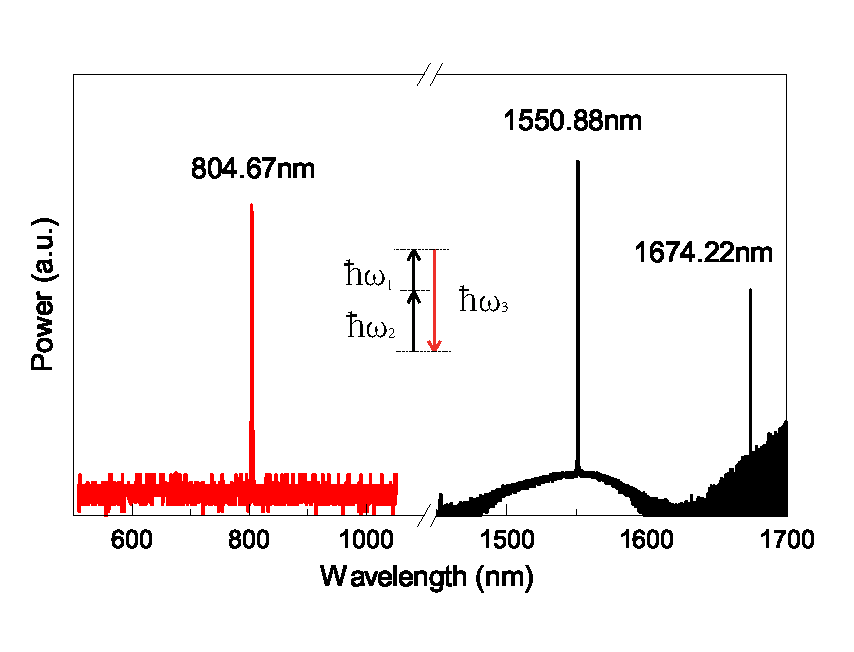
\includegraphics[width=8cm]{Fig4.eps}
\caption{\textbf{Measured spectra of second-order sum frequency generation (SFG). }The pump light ($\omega_1$) and Raman light ($\omega_2$) are summed to generate the SF signal ($\omega_3$).}
\label{pic:Fig4}
\end{figure}


%[More eg of SH; sum frequency]

 Sum frequency generation (SFG) can also take place when the pumped mode produce a Raman signal. Fig.\ref{pic:Fig4}b shows an SF signal and the corresponding pump and Raman spectrum.  The measured wavelengths satisfy the SFG relation $1/1550.88$ $\mathrm{nm} +1/1674.22$ $\mathrm{nm} = 1/804.63$ $\mathrm{nm}$, which is close to the measured SF wavelength 804.67 nm.

[Conclusion]




\bibliography{ref}
\end{document}

